%
% File mtsxiv.tex, a copy of eamt12.tex
%
% Contact: mlf@dlsi.ua.es

%%% To ease future customizations, various replaceables have been paramaterized
%%% as listed in the newcommands section

\documentclass[11pt]{article}
\usepackage{mtsxiv}
\usepackage{times}
\usepackage{latexsym}
\usepackage{url}
\setlength\titlebox{6.5cm}    % Expanding the titlebox
%%% YOUR PACKAGES BELOW THIS LINE %%%
\usepackage[utf8]{inputenc}
\usepackage{multirow} 
\usepackage[small,bf]{caption} 

\newcommand{\confname}{Machine Translation Summit XIV}
\newcommand{\website}{\protect\url{http://www.mtsummit2013.info/}}
\newcommand{\contactname}{research track co-chair Mikel L.\ Forcada}
\newcommand{\contactemail}{mlf@dlsi.ua.es} 
\newcommand{\conffilename}{mtsxiv}
\newcommand{\downloadsite}{\protect\url{http://www.mtsummit2013.info/}}
\newcommand{\paperlength}{$8$ (eight)}
\newcommand{\shortpaperlength}{$4$ (four)}

\usepackage{multibib}
\usepackage[comma]{natbib}
\usepackage{chapterbib}

\usepackage{lingmacros}
\usepackage{threeparttable}

\newcommand{\todo}[1]{\{\textbf{TODO: #1}\}}
\newcommand{\note}[1]{\{\textbf{Note: #1}\}}

\usepackage{fancyvrb} 
\DefineVerbatimEnvironment{outputExample}{Verbatim}{fontsize=\small}
\DefineVerbatimEnvironment{goldExample}{BVerbatim}{fontsize=\tiny}

\bibdata{mtsxivslsh}

\newcommand{\sentenceexample}[1]{{\small\enumsentence{#1}}}

\title{Shallow-transfer rule-based machine translation for the Western group of South Slavic languages}

\author{Hrvoje Peradin\\
  University of Zagreb\\
  Faculty of Science\\
  Department of Mathematics\\
  {\tt hperadin@gmail.com}  \And
  Filip Petkovski \\
  University of Zagreb\\
  Faculty of Electrical Engineering\\
  and Computer Science\\
  {\tt filip.petkovski@fer.hr}  \And
  Francis M. Tyers\\
  Dept. Lleng. i Sist. Inform.\\
  Universitat d'Alacant\\
  E-03899 Alacant\\
  {\tt ftyers@dlsi.ua.es}}

\date{}

\begin{document}
\maketitle
\begin{abstract}
The South Slavic languages, spoken mostly in the Balkans, make up one
of the three Slavic branches. The South Slavic branch is in turn
comprised of two subgroups, the Eastern subgroup containing Macedonian
and Bulgarian, and the western subgroup containing Serbo-Croatian
and Slovenian. This paper describes the development of a
bidirectional machine translation system for the western branch of
South-Slavic languages — Serbo-Croatian and Slovenian. Both
languages have a free word order, are highly inflected, and share a
great degree of mutual inteligibility. We give details on resources and
development methods used, as well as an evaluation, and
general directions for future work.
\end{abstract}

%\section{Credits}
%\todo{Credit where credit is due...}

% INTRODUCTION

\section{Introduction}

The South Slavic language branch, which is spoken mostly in the
Balkans, makes up one of the three Slavic branches. The South Slavic
branch itself is in turn comprised of two subgroups, the Eastern subgroup
containing Macedonian and Bulgarian, and the western subgroup
containing Serbo-Croatian and Slovenian.

The Serbo-Croatian (\texttt{hbs})\footnote{We use the term `Serbo-Croatian' as an abbreviation for
Bosnian-Croatian-Montenegrin-Serbian.} 
dialects are the native language of most people in Serbia, Croatia, 
Montenegro and Bosnia and Herzegovina. They were formed on the basis of the \emph{štokavian} dialects 
which got their name from the form \emph{što} (or \emph{šta}), which is used for the 
interrogative pronoun `what?'. A second group of dialects from the Serbo-Croatian language group 
is the Čakavian group spoken in western Croatia, Istria, the coast of Dalmatia, and some 
islands in the Adriatic. Like the štokavian dialects, the \emph{čakavian} dialects got their name 
from the form \emph{ča} used for the same interrogative pronoun. Finally, the third main group 
of Serbo-Croatian dialects, spoken in north-western Croatia, uses \emph{kaj} instead of \emph{što}, 
and is called \emph{kajkavian}.
An intermediate dialect between Serbo-Croatian, Bulgarian and Macedonian is the Torlakian dialect.
The three or four standardised varieties of Serbo-Croatian are all based on the štokavian dialect.

Slovenian (\texttt{slv}) is the native language of Slovenia, and is also spoken in the neighbouring areas in Italy and Austria. While Slovenian has many different dialects, it shares some features with the Kajkavian dialects spoken in Croatia. Although the speakers of the different Serbo-Croatian dialects can understand each other without any serious difficulties, a Serbo-Croatian speaker can have a difficult time understanding a speaker of a Slovenian dialect.

\begin{figure}
\centering
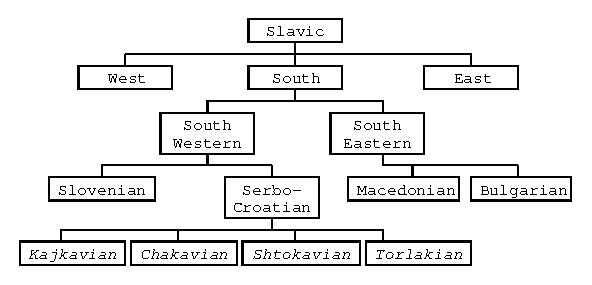
\includegraphics[width=0.5\textwidth]{images/chart.eps}
\caption{A traditional division of the South-Slavic languages. All four standard varieties
     of Serbo-Croatian (Bosnian, Croatian, Montenegrin, and Serbian) are based on the 
     štokavian dialect.}
\end{figure}

\begin{table*}
\centering
\begin{tabular}{lcccc}
  \hline
              &  \textbf{Bosnian} & \textbf{Croatian} & \textbf{Montenegrin} & \textbf{Serbian}\\
  \hline
 \textbf{Čakavian}  & - & -i-,-e-,-je- & - & -  \\
 \textbf{Kajkavian}  & - & -e-,-ie-,-ei,-i- & - & -  \\
 \textbf{Štokavian}  & -ije-,-je- & -ije-,-je-,-i- & -ije-,-je- & -e-,-ije-,-je-  \\
 \textbf{Torlakian}  & - & - & - & -e-  \\
\hline
\end{tabular}
\caption{Intersection of Serbo-Croatian languages and dialects. All four standard variants 
  are based on the štokavian dialect, but other dialects are considered to \emph{belong} to a 
  standard. The -ije-, -e-, and -i- correspond to the \emph{yat} reflex.}
\end{table*}

%% \begin{figure}

%% \todo{Venn diagram of Serbo-Croatian, Serbian, Croatian, Bosnian, Montenegrin, 
%% Neo-Štokavian, Čakavian, Kajkavian, Torlakian
%% Ekavian, Ijekavian, Ikavian}

%% \end{figure}



% DESIGN 
\section{Design}
\subsection{The Apertium platform}
\nocite{forcada2011apertium}
The Apertium\footnote{\url{http://wiki.apertium.org/}} platform is a
modular machine translation system. The typical core layout consists
of a letter transducer morphological lexicon\footnote{A list of
ordered pairs of word surface forms and their lemmatised
analyses.}. The transducer produces cohorts\footnote{A cohort 
consists of a surface form and one or more readings containing the lemma of the 
word and the morphological analysis.} which are then subjected to a
morphological disambiguation process.
%
Disambiguated readings are then looked up in the bilingual dictionary,
which gives the possible translations for each reading. These
are then passed through a lexical-selection module \citep{tyers12a}, 
which applies rules which select the most appropriate translation
for a given source-language context.
After lexical selection, the readings, which are now pairs of source
and target language lexical forms are passed through a 
syntactic transfer module that performs word reordering, deletions,
insertions, and basic syntactic chunking.
%
The final module is another letter transducer which generates
surface forms in the target language from the bilingual transfer
output cohorts.

\subsection{Constraint Grammar}
This language pair uses a Constraint Grammar (CG)
module\footnote{Implemented in the CG3 formalism, using the
  \texttt{vislcg3} compiler, available under GNU GPL. For a detailed
  reference see: \url{http://beta.visl.sdu.dk/cg3.html}} for
disambiguation. The CG formalism consists of hand-written rules that
are applied to a stream of tokens. Depending on the morphosyntactic
context of a given token the rules select or exclude readings of a
given surface form, or assign additional tags.


% DEVELOPMENT
\section{Development}

\subsection{Resources}
This language pair was developed with the
aid of on-line resources containing word definitions and flective
paradigms, such as \emph{Hrvatski jezični
  portal}\footnote{\url{http://hjp.srce.hr}} for the Serbo-Croatian side. For
the Slovenian side we used a similar online resource \emph{Slovar
  slovenskega knjižnega
  jezika},\footnote{\url{http://bos.zrc-sazu.si/sskj.html}} and the
\emph{Amebis Besana} flective
lexicon.\footnote{\url{http://besana.amebis.si/pregibanje/}}

The bilingual dictionary for the language pair was developed from scratch,
using the \emph{EUDict}\footnote{\url{http://eudict.com/}} online
dictionary and other online resources.
%\emph{Google Translate}\footnote{\url{http://translate.google.com/}}.

\subsection{Morphological analysis and generation}
The basis for this language pair are the morphological
lexicons for Serbo-Croatian (from
the language pair Serbo-Croatian--Macedonian, {\small{\tt apertium-hbs-mak}}) and Slovenian (from the
language pair Slovenian--Spanish, {\small{\tt apertium-slv-spa}}). Both
lexicons are written in the XML format of
\emph{lttoolbox}\footnote{\url{http://wiki.apertium.org/wiki/Lttoolbox}}
\cite{rojas2005construccion}, and were developed as parts of
their respective language pairs, during the Google Summer of Code
2011.\footnote{\url{http://code.google.com/soc/}} Since the lexicons
had been developed using different frequency lists, and slightly
different tagsets, they have been further trimmed and updated to
synchronise their coverage.

%wiktionaries and Wikipedia, as well as an SETimes corpus\footnote{\url{http://opus.lingfil.uu.se/SETIMES.php}} (\citealp{tyers2010south}) and a%corpus composed from the Serbian, Bosnian, Croatian and Serbo-Croatian Wikipedias.

%% Other resources for morphological analysis of Serbian and Croatian exist
%% (\citealp{vitas2004intex}, \citealp{vitas2003processing}, \citealp{agic2008improving}, \citealp{snajder08automatic}), 
%% to our knowledge there are none freely available for either Serbian, Bosnian or
%% Croatian. 


\begin{table}

\begin{center}
\begin{tabular}{|l|rrr|}
\hline
\textbf{Dictionary} & \textbf{Paradigms} & \textbf{Entries} & \textbf{Forms} \\
\hline
Serbo-Croatian &  1,033 & 13,206 & 233,878 \\
Slovenian &  1,909 & 13,383 & 147,580 \\
\hline
Bilingual &  69 &  16,434 & 70,787 \\
\hline
\end{tabular}
\caption{Statistics on number of lexicon entries for each of the dictionaries in the 
   system.}
\end{center}

\end{table}

\begin{table}
\begin{center}
\begin{tabular}{|l|rr|}
\hline
 \textbf{Type}      & \texttt{hbs}$\rightarrow$\texttt{slv} & \texttt{slv}$\rightarrow$\texttt{hbs}\\
\hline
Disambiguation      &     194              &     28 \\
Lexical selection   &     --            &  42 \\
Transfer            &                47 &  98 \\
\hline

\end{tabular}
 \caption{Statistics on the number of rules in each direction. For the lexical selection rules, 
   the number indicates that there are 42 rules for each of the three standard varieties currently
   supported.}
\end{center}
\end{table}

% EVALUATION 
\section{Evaluation}
% Hrvatski -> Slovenski
\begin{table}
\begin{tabular}{lrr}

\textbf{Language} & \textbf{SETimes} & \textbf{Europarl}\\
\hline
Serbo-Croatian & 85.41\% & -- \\
Slovenian &  -- & 95.50\%\\
\hline
\end{tabular}
\caption{ Statistics on number of lexicon entries for each of the
dictionaries in the system }
\label{table:coverage}
\end{table}


This sections covers the evaluation of the developed system. 
The system was tested by measuring the lexical coverage, and by performing
a qualitative and a quantitative evaluation. 

Lexical coverage was tested using existing free corpora, 
while the quantitative evaluation was performed on 100 postedited sentences (with 1,055 words in
total) from the Slovenian news portal 
Delo. \footnote{\url{http://www.delo.si/}}

Statistics on the size of the resulting lexicons are given in table
\ref{table:lexicons}, and the rule counts are listed in table
\ref{table:rules}. While the lexicons are evenly matched, the number
of rules is slightly in favour of the \texttt{hbs} side. This is due
to the fact that after the initial development phase additional work
has been done in the transfer module for the \texttt{slv}
$\rightarrow$ \texttt{hbs} direction, and the disambiguation and
lexical selection modules have been developed by native speakers of
Serbo-Croatian who are not fluent in Slovene.

\subsection{Lexical coverage}

Coverage for the Serbo-Croatian--Slovenian language pair was measured using both the SETimes \cite{tyers2010south} and Europarl \cite{koehn05a} corpora. 
We measured coverage naively, meaning that we assume a word is in our 
dictionaries if at least one of its surface forms is found in the corpus. 
We are aware of the shortcomings of such an evaluation framework, 
however we decided to use it because of its simplicity.

The Serbo-Croatian $\rightarrow$ Slovenian side was evaluated using the SETimes corpus.
As SETimes does not cover Slovenian
the Slovenian $\rightarrow$ Serbo-Croatian side was evaluated only on the EuroParl corpus. The results are shown in table \ref{table:coverage}.

\subsection{Quantitative}

The quantitative evaluation was performed by 5 articles
from the Slovenian news portal Delo.
The articles were translated from Slovenian using Apertium, and were later corrected by a human post-editor in order to get a correct translation.
The Word Error Rate (WER) was calculated
by counting the number of insertions, substitutions and deletions between the post-edited articles
and the original translation. We used the freely available \texttt{apertium-eval-translator} for calculating the WER 
and for bootstrap resampling \cite{koehn04}.
We also reported the percentage of out of vocabulary words (OOV), and the total number of words per article.
The results are given in table \ref{table:quantitative1}.

We also calculated both metrics for the output of Google Translate\footnote{\url{http://translate.google.com/}} 
and the results are presented in the same tables. Note that to compare the systems
we made two posteditions, one from the Apertium translation, and the other 
from the Google translation, so as not to bias the evaluation in either direction.

The post-editting evaluation shows comparable results for our system
and Google Translate according to WER and PER metrics.  The Slovenian
$\rightarrow$ Serbo-Croatian translation seems to be better than the
Serbo-Croatian $\rightarrow$ Slovenian one which is due to the fact
that more effort was put into developing the former direction.


% cp /path/to//apertium//trunk/apertium-eval-translator/WER.pl /path/to/bin
% perl apertium//trunk/apertium-eval-translator/bootstrap_resampling.pl -n 1000 -e /path/to//apertium//trunk/apertium-eval-translator/wer.sh -s SOURCE_FILE -t TEST_FILE -r REF_FILE

\begin{table*}
\begin{center}
\begin{tabular}{|l|r|rr||rr|}
   \hline
  \multirow{2}{*}{\textbf{Article}}  & \multirow{2}{*}{\textbf{Words}} & \multicolumn{2}{|c||}{\textbf{\%~OOV}} & \multicolumn{2}{c|}{\textbf{WER}}\\\cline{3-6}
                    &                & Apertium & Google &  Apertium & Google \\
   \hline
   \hline
  \texttt{maraton}  & 243            & 16.8     & --     & \textbf{[42.85, 47.92]} & [64.39, 74.56] \\
  \texttt{sonce}    & 169            & 17.7     & --     & \textbf{[32.65, 45.33]}    & [47.27, 58.62] \\
  \texttt{merkator} & 414            & 16.9     & --     & \textbf{[38.78, 48.14]}     & [56.13, 70.30] \\
  \texttt{volitve}  & 229            & 13.9     & --     & [37.81, 53.36]      & [46.66, 62.67] \\
%  \texttt{jame}     & 994            & 14.9     & --     & ??      & [57.28, 67.65] \\
                                                           % 49.57	
  \hline
  \hline
  \texttt{maraton}  & 245            & 37.7     & --     & [52.78, 56.25]           & [45.58, 63.87]\\
  \texttt{sonce}    & 171            & 17.5     & --     & [47.50, 62.79]    & [32.10, 58.49] \\
  \texttt{merkator} & 424            & 12.9     & --     & [45.78, 56.56]    & [48.46, 64.15] \\
  \texttt{volitve}  & 226            & 16.8     & --     & [47.00, 58.44]    & [38.09, 58.10]\\
%  \texttt{jame}     & 1,005          & 15.9     & --     & [??, ??]              & [??,??]\\

  \hline
\end{tabular}
 \caption{Results for Word Error Rate (WER) in the Slovenian$\rightarrow$Serbo-Croatian direction (top) and Serbo-Croatian$\rightarrow$Slovenian (bottom). Scores in bold show a statistically significant improvement over the other system according to bootstrap resampling at $p = 0.95$.}
\label{table:quantitative1}
\end{center}
\end{table*}




\subsection{Qualitative}
The biggest problems are currently caused by the incompleteness of our dictionaries.
The issues caused by OOV words are twofold.
The less important issue is the fact that the system is unable to provide a translation for the unknown words ---
although in many cases, such as with proper names, these may result in \emph{free rides}, that is the word
is the same in both languages.
However, the more important issue is that OOV words cause problems with disambiguation and transfer, since they
break long chains of words into smaller ones and drastically reduce context information. 

Next, we have seen that the number of disambiguation rules for
Slovenian is not sufficient for high-quality disambiguation.  The
constraint grammar for the Slovenian side was written based on the
constraint grammar for the Serbo-Croatian side, and it needs further
work.\footnote{An evaluation of a more extensive Constraint
  grammar for Croatian can be found in \cite{peradin2012towards}}

We have also noticed difficulties in the transfer because of the loose
grammar of both sides. Variations created by the free word order, and
long distance relationships between sentence constituents make it
difficult to write translation rules that cover a wide variety of
language constructs. Adding additional rules does not significantly
improve the performance of the system and OOV words make long transfer
rules irrelevant.

Finally, because of the short timeframe, and due to the fact no
reliable parallel corpus exists for this language pair,\footnote{There
is e.g. \url{http://opus.lingfil.uu.se/}, but it consists mostly of
texts from OpenSubtitles} we were unable to do much work on lexical selection.
Our lexical-selection module is the least developed part of our
system. We have not done any work on the Slovenian side and the number
of rules for the Serbo-Croatian side is small.



% CONCLUSIONS AND FUTURE WORK
\section{Future work}

The greatest difficulties for our system are caused by the long phrases present 
and the loose and free word order in the South Slavic languages.
Because of that, in future we plan to put more effort into dealing with those problems.
We are aware of the fact that it is difficult to write transfer rules between the two sides,
and we intend to address that issue by first improving the coverage of our dictionaries.

After expanding the dictionaries, we intend to put more time into developing the Slovenian constraint grammar,
and improve transfer by taking into account wider context.

We intend to work on more Slavic language pairs, including Serbo-Croatian--Russian,
and improve our existing ones, including Serbo-Croatian--Macedonian \citep{peradin12} using the 
resources and knowledge obtained by developing this language pair.

Finally, we will keep the resources updated based on the latest politico-linguistic developments,
and we will add the Montenegrin language once the standard is completely agreed on.


%mention different word order, long phrases, difficult to write rules for
%improve coverage, disambiguation (esp. for slv) and transfer rules
%work on more Slavic language pairs (e.g. hbs-rus)
%backport improvements in the HBS components to hbs-mak
%keep up-to-date with latest politico-linguistic developments. Add in
% Montenegrin when the standard is agreed on.
%small timeframe, disambiguation and transfer rudimentary

\section{Conclusions}

This language pair was an encouraging take on a pair of closely
related South-Slavic languages, and represents a satisfying conclusion
to an MT chain of neighbouring languages (the pairs Serbo-Croatian--Macedonian 
and Macedonian--Bulgarian are also available in Apertium). While we are aware that it
is still in its infancy, and has many flaws, it is a valuable
free/open-source resource, and will serve as another solid ground for NLP
in this language group.




\section*{Acknowledgements}

The development of this language pair was funded as a part of the
Google Summer of Code.\footnote{\url{http://code.google.com/soc/}}
Many thanks to the language pair co-author Ale\v{s} Horvat and his
mentor Jernej Vičič, and other Apertium contributors for their
invaluable help and support.

%\nocite{*}
%\bibliographystyle{mtsxiv}
\bibliographystyle{apalike}
\bibliography{mtsxivslsh}

\end{document}

%% \begin{thebibliography}{}

%% \bibitem[\protect\citename{Aho and Ullman}1972]{Aho:72}
%% Aho, Alfred~V. and Jeffrey~D. Ullman.
%% \newblock 1972.
%% \newblock {\em The Theory of Parsing, Translation and Compiling}, volume~1.
%% \newblock Prentice-{Hall}, Englewood Cliffs, NJ.

%% \bibitem[\protect\citename{{American Psychological Association}}1983]{APA:83}
%% {American Psychological Association}.
%% \newblock 1983.
%% \newblock {\em Publications Manual}.
%% \newblock American Psychological Association, Washington, DC.

%% \bibitem[\protect\citename{{Association for Computing Machinery}}1983]{ACM:83}
%% {Association for Computing Machinery}.
%% \newblock 1983.
%% \newblock {\em Computing Reviews}, 24(11):503--512.

%% \bibitem[\protect\citename{Chandra \bgroup et al.\egroup }1981]{Chandra:81}
%% Chandra, Ashok~K., Dexter~C. Kozen, and Larry~J. Stockmeyer.
%% \newblock 1981.
%% \newblock Alternation.
%% \newblock {\em Journal of the Asso\-ciation for Computing Machinery},
%%   28(1):114--133.

%% \bibitem[\protect\citename{Gledson and Keane}2008a]{Gledson:08homog}
%% Gledson, Anne, and John Keane. 
%% \newblock 2008a. 
%% \newblock Measuring Topic Homogeneity and its Application to Dictionary-Based Word-Sense Disambiguation. 
%% \newblock {\em Coling 2008, 22nd International Conference on Computational Linguistics}, Manchester, UK.
%% \newblock 273--280.
%% \bibitem[\protect\citename{Gledson and Keane}2008b]{Gledson:08websearch}
%% Gledson, Anne, and John Keane. 
%% \newblock 2008b. 
%% \newblock Using Web-Search Results to Measure Word-group Similarity. \newblock {\em Coling 2008, 22nd International Conference on Computational Linguistics}, Manchester, UK.
%% \newblock 281--288.
%% \bibitem[\protect\citename{Gusfield}1997]{Gusfield:97}
%% Gusfield, Dan.
%% \newblock 1997.
%% \newblock {\em Algorithms on Strings, Trees and Sequences}.
%% \newblock Cambridge University Press, Cambridge, UK.

%% \bibitem[\protect\citename{Tam and Schultz}2006]{Tam:06}
%% Tam, Yik-Cheung and Tanja Schultz.
%% \newblock 2006. 
%% \newblock Unsupervised Language Model Adaptation Using
%%   \nobreak{Latent} Semantic Marginals.
%% \newblock {\em Interspeech 2006 -- ICSLP, Ninth International Conference on Spoken Language Processing}, 
%% Pittsburgh, Pennsylvania, paper 1705-Thu1A2O.2. 

%% \bibitem[\protect\citename{Tam and Schultz}2007]{Tam:07}
%% Tam, Yik-Cheung and Tanja Schultz.
%% \newblock 2007.
%% \newblock Correlated \nobreak{Latent} Semantic Model for
%%   Unsupervised Language Model Adaptation.
%% \newblock {\em Proceedings of ICASSP 2007, International Conference on 
%%   Acoustics, Speech, and Signal Processing}, Honolulu, Hawaii, Vol. IV, 41--44.

%% \end{thebibliography}


